\newpage
\chapter{TINJAUAN PUSTAKA} \label{Bab II}

\section{Tinjauan Pustaka} \label{II.Tinjauan}
Tinjauan pustaka dilakukan untuk memperoleh landasan teoritis dan empiris yang mendukung penelitian ini. Berbagai studi terdahulu dijadikan acuan dalam mengembangkan sistem informasi penerimaan mahasiswa baru (PMB) berbasis web yang terintegrasi dan sesuai dengan kebutuhan pengguna. Ringkasan beberapa penelitian yang relevan disajikan pada Tabel \ref{table:2.literasi} di bawah ini:\par

\begin{longtable}{|b{0.03\textwidth}|p{0.14\textwidth}|p{0.18\textwidth}|p{0.1\textwidth}|p{0.18\textwidth}|p{0.18\textwidth}|}
	\caption{Daftar Jurnal Terkait}
	\label{table:2.literasi}\\
	\hline
	\textbf{No.} & \textbf{Penulis [Tahun] [Judul]} & \textbf{Permasalahan dan Tujuan} & \textbf{Metode} & \textbf{Kontribusi} & \textbf{Kekurangan} \\
	\hline
	\endfirsthead
	\hline
	\textbf{No.} & \textbf{Penulis [Tahun] [Judul]} & \textbf{Permasalahan dan Tujuan} & \textbf{Metode} & \textbf{Kontribusi} & \textbf{Kekurangan} \\
	\hline
	\endhead
	1 & Nugraha, D., Fitriani, A., \& Sari, R. [2024] [Rancang Bangun Sistem Informasi PMB Berbasis Web Menggunakan Laravel 8 di Politeknik Indorama] \cite{nugraha2024rancang} & Pengembangan website PMB di Politeknik Indorama awalnya dilakukan semi-manual dan tidak efisien. Tujuan: membuat sistem PMB Laravel 8 yang efisiensi input \& validasi data. & Laravel 8, MySQL, MVC & Sistem mampu menangani proses pendaftaran secara digital dengan tampilan sederhana dan pemrosesan cepat. & Belum ada integrasi dengan sistem pembayaran otomatis (misal BRIVA), dan tidak mendukung manajemen data dinamis seperti gelombang \& harga. \\
	\hline
	2 & Novianto, M. A. [2022] [Analisis dan Implementasi RESTful API guna Pengembangan Sistem Informasi Akademik Perguruan Tinggi] \cite{novianto2023analisis} & Sistem akademik tidak terintegrasi dan lambat. Tujuan: menerapkan REST API dengan Spring agar sistem lebih modular dan \textit{scalable}. & Spring Framework, RESTful API & Sistem dapat digunakan sebagai fondasi pengembangan modul seperti PMB yang lebih fleksibel dan mudah diintegrasikan. & Fokus masih pada API \textit{backend}, belum mencakup UI, notifikasi email, atau pengelolaan PMB secara \textit{end-to-end}. \\
	\hline
	3 & Adji, L. S., \& Mailoa, E. [2024] [Pembuatan REST API Manajemen Data Karyawan Berbasis Website Menggunakan Spring Boot] \cite{adji2024pembuatan} & Sistem pengelolaan data karyawan kurang efisien. Tujuan: membangun REST API menggunakan Spring Boot untuk proses CRUD yang rapi dan aman. & Spring Boot, PostgreSQL, REST API & Memberikan arsitektur REST API yang bisa diadaptasi untuk PMB berbasis Spring dengan keamanan dan efisiensi tinggi. & Fokus studi bukan pada PMB; tidak membahas UI/UX, soal ujian, atau sistem pembayaran otomatis. \\
	\hline
	4 & Yulianto, R. [2024] [Performance Comparison Analysis of SpringBoot and Laravel Frameworks Using API Web Service] \cite{yulianto2024performance} & Perbandingan performa antara dua framework populer. Tujuan: menganalisis performa, respons API, dan efisiensi masing-masing framework. & Laravel vs SpringBoot, Postman, Benchmark API & Memberi \textit{insight} teknis mendalam untuk memilih framework terbaik dalam membangun sistem seperti PMB. & Tidak membahas implementasi nyata sistem PMB; hanya membandingkan performa framework. \\
	\hline
	5 & Rohman, T. W., et al. [2025] [Rancang Bangun Sistem Pendaftaran Siswa Baru SMK Citra Negara Depok Menggunakan Metode Waterfall] \cite{rohman2025rancang} & Sistem PPDB SMK sebelumnya tidak terdigitalisasi. Tujuan: membangun sistem Laravel 8 untuk digitalisasi penuh proses pendaftaran. & Laravel 8, MySQL, Blade & Menyediakan contoh penerapan Laravel dalam konteks PPDB (setara PMB) dengan form pendaftaran, upload berkas, dan validasi. & Tidak ada fitur integrasi BRIVA, notifikasi email, atau modul admin yang bisa mengatur gelombang \& formulir secara dinamis. \\
	\hline
\end{longtable}

Beberapa penelitian sebelumnya menjadi dasar dalam pengembangan sistem Penerimaan Mahasiswa Baru (PMB) berbasis web ini. Pada penelitian Nugraha et al. (2024) membangun sistem PMB berbasis Laravel 8 untuk mempermudah proses pendaftaran yang sebelumnya semi-manual. Sistem tersebut efisien, namun belum mendukung pembayaran otomatis.\par

Novianto (2022) menerapkan RESTful API berbasis Spring Framework untuk meningkatkan integrasi dan skalabilitas sistem akademik. Meski hasilnya modular dan stabil, penelitian ini belum membahas antarmuka pengguna dan fitur notifikasi. Sementara itu, Adji \& Mailoa (2024) membuat REST API dengan Spring Boot untuk manajemen data karyawan yang lebih aman dan efisien, tetapi belum mencakup fitur \textit{front-end} atau proses seleksi peserta seperti pada PMB.\par

Selanjutnya, Yulianto (2024) membandingkan performa Laravel dan Spring Boot dan menemukan bahwa Spring Boot lebih unggul dari sisi kecepatan dan skalabilitas. Namun, penelitian tersebut hanya bersifat analisis performa tanpa penerapan sistem nyata. Adapun Rohman et al. (2025) mengembangkan sistem PPDB berbasis Laravel 8 dengan fitur pendaftaran dan validasi, tetapi belum dilengkapi pembayaran otomatis, notifikasi email, atau pengaturan jadwal.\par

Dari kelima penelitian itu, dapat disimpulkan bahwa belum ada sistem PMB yang benar-benar terintegrasi penuh, terutama dalam hal pembayaran otomatis (BRIVA), ujian daring, notifikasi email, dan manajemen konten dinamis. Selain itu, belum ada yang menggunakan metode \textit{Prototype} untuk menyesuaikan sistem berdasarkan umpan balik pengguna. Karena itu, penelitian ini mengembangkan sistem PMB berbasis Spring Framework dengan pendekatan \textit{Prototype}, agar hasilnya lebih interaktif, efisien, dan sesuai kebutuhan Universitas HKBP Nommensen.\par

\section{Dasar Teori} \label{II.Teori}

\subsection{Manajemen Proyek Teknologi Informasi} \label{II.ManajemenProyekTI}
Manajemen proyek teknologi informasi (TI) merupakan penerapan ilmu dan teknik untuk merencanakan, melaksanakan, memantau, dan mengendalikan proyek berbasis TI agar tujuan organisasi tercapai secara efektif dan efisien \cite{witania2016analisis}. Berbagai metode manajemen proyek seperti \textit{Waterfall} dan \textit{Agile} diterapkan sesuai dengan kebutuhan organisasi \cite{witania2016analisis}. Namun dalam praktiknya, implementasi proyek TI kerap menghadapi tantangan seperti koordinasi tim dan pengendalian perubahan, terutama dalam situasi dinamis seperti masa pandemi \cite{pradana2020tantangan}.\par

\subsection{Aplikasi Penerimaan Mahasiswa Baru} \label{II.AplikasiPMB}
Aplikasi berbasis web untuk proses penerimaan mahasiswa baru dirancang untuk memfasilitasi pendaftaran daring, pengelolaan data calon peserta, dan administrasi secara efisien. Sistem ini mengintegrasikan komponen seperti formulir \textit{online}, validasi dokumen, pengelolaan gelombang, dan notifikasi otomatis melalui antarmuka web. Keunggulan utama dari sistem ini adalah efisiensi waktu pendaftaran, kemudahan akses, dan pengelolaan data yang lebih terstruktur dan akurat \cite{widiyatmoko2024development}.\par

\subsection{Model Pengembangan Perangkat Lunak} \label{II.ModelPengembangan}

\subsubsection{Metode Prototype} \label{II.MetodePrototype}
Metode \textit{Prototype} merupakan pendekatan dalam pengembangan perangkat lunak yang menitikberatkan pada pembuatan model awal dari sistem yang akan dibangun. Model ini berfungsi sebagai gambaran awal agar pengguna dapat memahami bentuk dan fungsi dasar sistem sejak tahap awal. Melalui \textit{prototype} tersebut, pengguna dapat memberikan masukan langsung terhadap tampilan maupun alur sistem, sehingga pengembang dapat melakukan penyesuaian sebelum sistem dikembangkan secara penuh. Berbeda dengan model \textit{Waterfall} yang berjalan secara berurutan dan jarang memungkinkan perubahan di tengah proses, metode \textit{Prototype} bersifat lebih fleksibel dan interaktif \cite{nurfauziah2023perbandingan}. Setiap tahap dapat diulang sesuai kebutuhan hingga sistem benar-benar sesuai dengan harapan pengguna. Penelitian menyebutkan bahwa proses \textit{prototyping} mencakup lima aspek penting, yaitu tujuan, ruang lingkup, media, penggunaan oleh pemangku kepentingan, serta strategi eksplorasi. Kelima aspek tersebut membantu memastikan bahwa pengembangan sistem berjalan selaras dengan kebutuhan dan pengalaman pengguna \cite{bjarnason2023empirically}.\par

\begin{figure}[H]
	\centering
	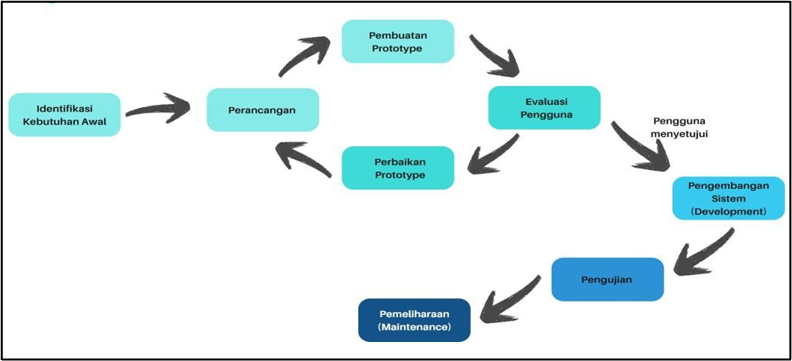
\includegraphics[width=0.7\textwidth]{figure/metode-prototype.png}
	\caption{Metode Prototype}
	\label{fig:2.metodeprototype}
	{\footnotesize Sumber: Bjarnason et al. \cite{bjarnason2023empirically}}
\end{figure}

Menurut Bjarnason et al. \cite{bjarnason2023empirically}, metode \textit{Prototype} terdiri dari beberapa tahap yang dilakukan secara iteratif untuk memastikan sistem yang dikembangkan sesuai dengan kebutuhan pengguna. Setiap tahap memungkinkan adanya umpan balik yang cepat agar sistem dapat diperbaiki sebelum tahap implementasi akhir. Adapun tahapan-tahapan utama dalam metode ini adalah sebagai berikut:\par

\begin{enumerate}[noitemsep]
	\item \textbf{Komunikasi (\textit{Communication})}\\
	Tahap awal bertujuan untuk mengidentifikasi kebutuhan pengguna melalui diskusi, wawancara, atau observasi. Aktivitas ini membantu pengembang memahami permasalahan dan ekspektasi pengguna terhadap sistem yang akan dibuat.
	\item \textbf{Perancangan Cepat (\textit{Quick Design})}\\
	Pada tahap ini dibuat rancangan awal sistem dalam bentuk sketsa, diagram alur, atau model antarmuka sederhana. Rancangan ini digunakan untuk menggambarkan gambaran umum sistem kepada pengguna sebelum dilakukan pengembangan lebih lanjut.
	\item \textbf{Pembuatan Prototype (\textit{Building Prototype})}\\
	Rancangan awal kemudian dikembangkan menjadi \textit{prototype} sederhana yang mewakili fungsi utama sistem. Tujuan dari tahap ini bukan untuk menghasilkan produk akhir, melainkan alat bantu evaluasi dan validasi kebutuhan.
	\item \textbf{Evaluasi oleh Pengguna (\textit{User Evaluation})}\\
	\textit{Prototype} diuji secara langsung oleh pengguna untuk memperoleh umpan balik mengenai fungsionalitas, tampilan, dan kemudahan penggunaan. Hasil evaluasi digunakan untuk memperbaiki rancangan sistem.
	\item \textbf{Perbaikan Prototype (\textit{Refinement})}\\
	Berdasarkan masukan pengguna, \textit{prototype} diperbarui agar lebih sesuai dengan kebutuhan yang sebenarnya. Proses ini dapat dilakukan berulang kali sampai sistem dinilai memuaskan.
	\item \textbf{Implementasi dan Pengujian Akhir (\textit{Implementation and Final Testing})}\\
	Setelah \textit{prototype} akhir disetujui, sistem dikembangkan secara penuh dan diuji secara menyeluruh menggunakan metode yang sesuai, seperti \textit{black-box testing} atau \textit{usability testing}, guna memastikan fungsionalitas berjalan dengan baik.
\end{enumerate}

\subsubsection{\textit{Evolutionary Prototyping}} \label{II.EvolutionaryPrototyping}
Dalam konteks pengembangan perangkat lunak, metode \textit{Prototype} terbagi menjadi dua pendekatan utama, yaitu \textit{Throwaway Prototyping} dan \textit{Evolutionary Prototyping} \cite{crinnion1991evolutionary}. Pada pendekatan \textit{throwaway}, \textit{prototype} yang dibuat hanya berfungsi sebagai alat eksplorasi kebutuhan dan akan dibuang setelah kebutuhan terkonfirmasi, kemudian sistem final dibangun dari awal. Sebaliknya, pada pendekatan \textit{evolutionary}, \textit{prototype} yang dibangun tidak dibuang, melainkan terus disempurnakan secara bertahap hingga menjadi sistem akhir yang siap digunakan.\par

Menurut Crinnion \cite{crinnion1991evolutionary}, \textit{Evolutionary Prototyping} merupakan pendekatan pengembangan perangkat lunak yang menitikberatkan pada pembuatan \textit{prototype} secara terstruktur dan melakukan penyempurnaan secara berkelanjutan. \textit{Prototype} awal yang dibangun menjadi inti dari sistem baru, dan seluruh perbaikan serta penambahan kebutuhan dilakukan di atas fondasi tersebut. Pendekatan ini mengakui bahwa tidak semua kebutuhan dapat dipahami sejak awal, sehingga hanya fitur-fitur yang telah dipahami dengan baik yang dikembangkan terlebih dahulu \cite{davis1992operational}.\par

Davis \cite{davis1992operational} menambahkan bahwa \textit{Evolutionary Prototyping} sangat efektif untuk sistem yang kompleks dan memiliki kebutuhan yang belum sepenuhnya diketahui di awal. Pengembang dapat memfokuskan diri pada bagian-bagian sistem yang dipahami dengan baik, sementara bagian lainnya dikembangkan pada iterasi berikutnya berdasarkan umpan balik pengguna. Software Productivity Consortium \cite{spc1997erd} menegaskan bahwa pendekatan ini memungkinkan evolusi berkelanjutan terhadap kapabilitas sistem sebagai respons cepat terhadap perubahan kebutuhan pengguna dan teknologi.\par

Berbeda dengan metode \textit{Prototype} konvensional yang bersifat umum, \textit{Evolutionary Prototyping} secara eksplisit membagi pengembangan ke dalam beberapa iterasi. Setiap iterasi menghasilkan versi sistem yang fungsional dan dapat digunakan, bukan sekadar \textit{mockup} atau model. Keunggulan utama pendekatan ini adalah sebagai berikut:\par

\begin{enumerate}[noitemsep]
	\item \textbf{Sistem selalu fungsional} -- setiap iterasi menghasilkan versi yang dapat digunakan, meskipun belum lengkap fiturnya.
	\item \textbf{Risiko diminimalkan} -- fitur yang belum dipahami dengan baik tidak dipaksakan untuk dikembangkan, sehingga mengurangi risiko kesalahan besar.
	\item \textbf{Umpan balik berkelanjutan} -- pengguna dapat mengevaluasi sistem secara langsung di setiap iterasi dan memberikan masukan untuk perbaikan.
	\item \textbf{Efisien untuk pengembang tunggal} -- tidak memerlukan tim besar seperti \textit{Agile}/Scrum, cukup satu pengembang yang membangun secara bertahap.
\end{enumerate}

\begin{figure}[H]
	\centering
	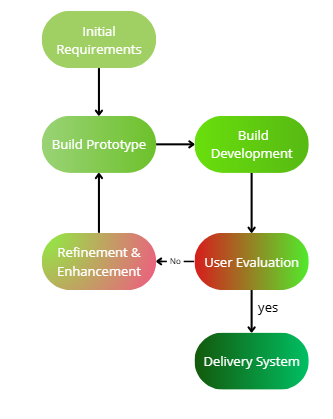
\includegraphics[width=0.75\textwidth]{figure/evolutionary-prototyping.png}
	\caption{Alur Metode \textit{Evolutionary Prototyping}}
	\label{fig:2.evolutionaryprototyping}
	{\footnotesize Sumber: Diadaptasi dari Davis \cite{davis1992operational}}
\end{figure}

Tahapan dalam \textit{Evolutionary Prototyping} menurut Crinnion \cite{crinnion1991evolutionary} dan Davis \cite{davis1992operational} meliputi:\par

\begin{enumerate}[noitemsep]
	\item \textbf{Analisis Kebutuhan Awal (\textit{Initial Requirements})}\\
	Mengidentifikasi kebutuhan inti yang telah dipahami dengan baik. Kebutuhan yang belum jelas ditandai untuk dikembangkan pada iterasi selanjutnya.
	\item \textbf{Pembangunan Prototype Awal (\textit{Build Initial Prototype})}\\
	Membangun \textit{prototype} fungsional berdasarkan kebutuhan inti. \textit{Prototype} ini bukan \textit{mockup}, melainkan sistem yang benar-benar dapat dijalankan.
	\item \textbf{Evaluasi Pengguna (\textit{User Evaluation})}\\
	Pengguna menguji \textit{prototype} dan memberikan umpan balik mengenai fungsionalitas, kekurangan, serta kebutuhan tambahan.
	\item \textbf{Penyempurnaan dan Penambahan Fitur (\textit{Refine and Extend})}\\
	Berdasarkan umpan balik, pengembang memperbaiki \textit{prototype} dan menambahkan fitur baru. Proses ini membentuk iterasi baru.
	\item \textbf{Iterasi Berulang (\textit{Iterate})}\\
	Tahap 3 dan 4 diulang hingga sistem memenuhi seluruh kebutuhan pengguna dan dianggap layak sebagai sistem final.
\end{enumerate}

Dengan karakteristik tersebut, \textit{Evolutionary Prototyping} sangat cocok diterapkan pada pengembangan sistem yang bersifat kompleks, memiliki banyak modul, dan dikerjakan secara bertahap oleh satu pengembang---seperti pengembangan sistem PMB dalam penelitian ini.\par

\subsection{\textit{Object-Oriented Programming} (OOP) dalam Java} \label{II.OOPJava}
Pemrograman berorientasi objek (\textit{Object-Oriented Programming}/OOP) merupakan paradigma yang memandang perangkat lunak sebagai kumpulan objek yang saling berinteraksi. Setiap objek memiliki atribut dan metode yang merepresentasikan data serta perilaku dalam satu kesatuan. Pendekatan ini berlandaskan pada empat prinsip utama, yaitu \textit{encapsulation} (pengemasan data dan perilaku dalam satu entitas), \textit{inheritance} (pewarisan sifat dari kelas induk ke kelas turunan), \textit{polymorphism} (kemampuan objek untuk berperilaku berbeda tergantung konteks), dan \textit{abstraction} (penyembunyian detail implementasi agar fokus pada fungsi utama).\par

Paradigma OOP memberikan cara yang efektif untuk merancang perangkat lunak yang terstruktur dan mudah dikembangkan karena tanggung jawab sistem dibagi menjadi kelas-kelas yang saling berhubungan namun independen \cite{parmar2024survey}. Penelitian lain menambahkan bahwa pendekatan ini mempermudah pengelolaan sistem berskala besar, sebab setiap komponen dapat diuji dan diperbarui tanpa mengganggu bagian lain \cite{nagineni2021research}.\par

Bahasa pemrograman Java menjadi salah satu implementasi paling populer dari konsep OOP. Java dikenal karena sifatnya yang \textit{platform independent} melalui prinsip ``\textit{Write Once, Run Anywhere}''. Selain itu, Java dilengkapi fitur \textit{exception handling} untuk menangani kesalahan saat \textit{runtime} dan \textit{garbage collection} untuk pengelolaan memori otomatis, yang menjadikan pengembangan perangkat lunak lebih stabil dan efisien. Penerapan konsep OOP pada Java memungkinkan rancangan kode yang modular, mudah dirawat, serta fleksibel untuk dikembangkan lebih lanjut \cite{fadillah2023features}.\par

\subsection{\textit{Model--View--Controller}} \label{II.MVC}
\textit{Model--View--Controller} (MVC) merupakan pola arsitektur perangkat lunak yang membagi sistem menjadi tiga komponen utama, yaitu \textit{Model}, \textit{View}, dan \textit{Controller}. \textit{Model} bertanggung jawab terhadap pengelolaan data serta logika bisnis, \textit{View} menampilkan data dalam bentuk antarmuka pengguna, sedangkan \textit{Controller} mengatur aliran data dan interaksi antara \textit{Model} dan \textit{View}.\par

Menurut Ismail \cite{ismail2023development}, penerapan pola MVC dalam pengembangan aplikasi web memberikan kejelasan struktur dan meningkatkan efisiensi pengelolaan kode karena setiap komponen memiliki tanggung jawab yang terpisah. Sementara itu, penelitian oleh Necula \cite{necula2024exploring} menegaskan bahwa arsitektur MVC meningkatkan \textit{scalability}, \textit{reusability}, serta \textit{maintainability} pada aplikasi web interaktif.\par

\begin{figure}[H]
	\centering
	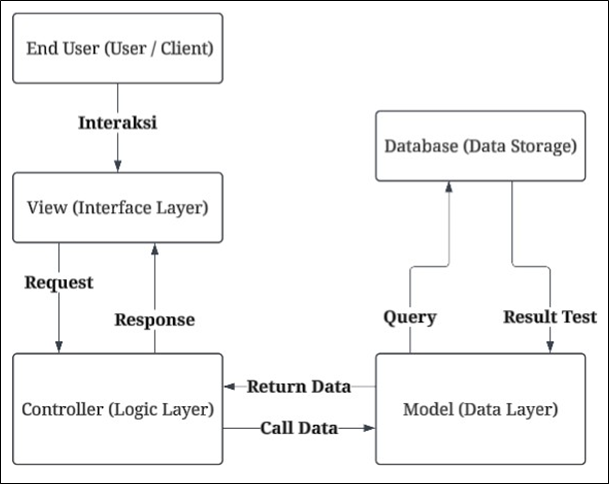
\includegraphics[width=0.6\textwidth]{figure/mvc-diagram.png}
	\caption{Diagram Umum Arsitektur \textit{Model--View--Controller} (MVC)}
	\label{fig:2.mvc}
\end{figure}

Arsitektur MVC memisahkan setiap tanggung jawab sistem agar mudah dikembangkan, diuji, serta dipelihara. Pola ini banyak digunakan pada framework modern seperti Spring Boot, Laravel, dan Django karena kemampuannya dalam menjaga modularitas dan fleksibilitas sistem.\par

\subsection{Spring Framework} \label{II.SpringFramework}
Spring Framework merupakan kerangka kerja \textit{open-source} berbasis Java yang dirancang untuk pengembangan aplikasi berskala besar dengan arsitektur yang modular, terstruktur, dan mudah dikelola \cite{sargunakumar2024spring}. Framework ini menyediakan berbagai modul pendukung, seperti Spring Boot yang menyederhanakan konfigurasi dan mempercepat proses pengembangan, serta Spring Security yang menangani autentikasi dan otorisasi pengguna. Dalam penerapannya, Spring Framework memungkinkan pengembang membangun API secara efisien, mengelola integrasi dengan basis data seperti MySQL atau PostgreSQL, serta memisahkan tanggung jawab sistem ke dalam lapisan \textit{controller}, \textit{service}, dan \textit{repository}. Pendekatan ini membantu menjaga kode tetap rapi, mudah diuji, serta memudahkan pemeliharaan saat terjadi perubahan kebutuhan aplikasi.\par

\subsection{\textit{HyperText Markup Language} (HTML) dan \textit{Cascading Style Sheets} (CSS)} \label{II.HTMLCSS}
\textit{HyperText Markup Language} (HTML) digunakan untuk membangun struktur dasar halaman web dengan menyusun elemen seperti formulir, tombol, maupun kolom \textit{input}. Bahasa \textit{markup} ini menentukan bagaimana konten ditampilkan secara semantik di peramban (\textit{browser}), sehingga menjadi fondasi utama dalam pembuatan antarmuka pengguna \cite{jain2024modern}. Sementara itu, \textit{Cascading Style Sheets} (CSS) berperan dalam mengatur tampilan visual dari elemen-elemen HTML, mencakup tata letak, warna, margin, padding, jenis dan ukuran huruf, serta pengaturan responsivitas agar halaman tetap nyaman diakses dari berbagai perangkat \cite{jain2024modern}. Kombinasi antara HTML dan CSS memungkinkan perancang web menghasilkan tampilan antarmuka yang terstruktur, konsisten, dan menarik secara visual. Penggunaan kedua teknologi ini secara tepat juga dapat meningkatkan kenyamanan serta pengalaman pengguna dalam berinteraksi dengan sistem yang dikembangkan.\par

\subsection{\textit{Database} Relasional (MySQL)} \label{II.MySQL}
\textit{Database} relasional merupakan sistem penyimpanan data yang menyusun informasi dalam bentuk tabel-tabel yang saling berhubungan. Setiap tabel berisi kolom dan baris yang merepresentasikan atribut serta entitas data, dan keterkaitannya diatur melalui relasi seperti \textit{primary key} dan \textit{foreign key} \cite{esakkirajan2016fundamentals}. Sistem ini biasanya digunakan untuk mengelola data terstruktur secara efisien, mulai dari penyimpanan hingga pengolahan dan penampilan informasi. Pengelolaan dilakukan menggunakan bahasa SQL (\textit{Structured Query Language}), dengan perintah dasar seperti \texttt{SELECT} untuk menampilkan data, \texttt{INSERT} untuk menambah data, \texttt{UPDATE} untuk mengubah data, dan \texttt{DELETE} untuk menghapus data. Struktur yang teratur membuat \textit{database} relasional banyak diterapkan dalam berbagai sistem informasi modern.\par

\textit{Entity--Relationship Diagram} (ERD) digunakan untuk memodelkan hubungan antarentitas dalam sistem basis data. Menurut penelitian, ERD berperan penting dalam menggambarkan struktur logis data serta hubungan antarobjek sehingga mempermudah proses perancangan dan implementasi basis data yang konsisten \cite{song1995comparative}.\par

\begin{longtable}{|p{0.35\textwidth}|p{0.55\textwidth}|}
	\caption{Simbol ER Diagram}
	\label{table:2.simbolERD}\\
	\hline
	\textbf{Simbol} & \textbf{Deskripsi} \\
	\hline
	\endfirsthead
	\hline
	\textbf{Simbol} & \textbf{Deskripsi} \\
	\hline
	\endhead
	Entitas (Persegi panjang) & Menunjukkan objek utama yang datanya disimpan, seperti pengguna atau transaksi. \\
	\hline
	Atribut (Oval) & Menjelaskan properti atau karakteristik dari suatu entitas, misalnya nama atau tanggal. \\
	\hline
	\textit{Primary Key} (Oval bergaris bawah) & Atribut unik yang digunakan untuk mengidentifikasi setiap data secara spesifik. \\
	\hline
	\textit{Multivalued Attribute} (Oval ganda) & Atribut yang dapat memiliki lebih dari satu nilai, misalnya nomor telepon. \\
	\hline
	Relasi (Belah ketupat) & Menunjukkan hubungan antarentitas, seperti ``memiliki'' atau ``mengelola''. \\
	\hline
	Kardinalitas (\textit{Multiplicity}) & Menggambarkan jumlah keterhubungan antarentitas, seperti satu-ke-banyak atau banyak-ke-banyak. \\
	\hline
	\textit{Weak Entity} (Persegi panjang ganda) & Entitas yang tidak dapat berdiri sendiri tanpa bergantung pada entitas lain karena tidak memiliki atribut kunci unik. \\
	\hline
	\textit{Identifying Relationship} (Belah ketupat ganda) & Relasi yang menghubungkan entitas lemah dengan entitas kuat, menandakan ketergantungan eksistensial antara keduanya. \\
	\hline
\end{longtable}

\subsection{Pengujian Sistem} \label{II.PengujianSistem}
Pengujian sistem merupakan tahap penting dalam pengembangan perangkat lunak untuk memastikan seluruh fungsi berjalan sesuai kebutuhan serta memberikan pengalaman pengguna yang optimal. Beberapa metode yang umum digunakan antara lain \textit{Black-box Testing}, \textit{Usability Testing} (\textit{System Usability Scale}/SUS), dan \textit{Integration Testing}.\par

\subsubsection{\textit{Blackbox Test}} \label{II.BlackboxTest}
Metode \textit{Black-box} berfokus pada pengujian fungsionalitas perangkat lunak tanpa melihat struktur internal atau kode program. Pendekatan ini menilai apakah keluaran sistem sesuai dengan masukan yang diberikan pengguna. Contohnya mencakup pengujian validasi \textit{input}, navigasi menu, serta proses autentikasi. Penelitian menunjukkan bahwa penerapan metode ini dengan acuan standar ISO/IEC 25010 dapat membantu memastikan kualitas fungsionalitas perangkat lunak berjalan sesuai harapan \cite{buana2022pengujian}.\par

Ada berbagai teknik yang digunakan dalam \textit{Black-Box Testing}, antara lain \cite{santi2022blackbox}:\par
\begin{enumerate}[noitemsep]
	\item \textit{Equivalence Partitioning} (ECP): membagi domain \textit{input} menjadi beberapa kelas ekivalen (valid dan invalid) sehingga pengujian dapat dilakukan secara efisien tanpa menguji semua kemungkinan \textit{input}.
	\item \textit{Boundary Value Analysis} (BVA): menguji nilai-nilai di sekitar batas domain \textit{input} karena kesalahan sering muncul pada titik ekstrem.
	\item \textit{Decision Table Testing}: menggunakan tabel keputusan untuk menggambarkan kombinasi kondisi \textit{input} dan aksi yang diharapkan.
	\item \textit{State Transition Testing}: memeriksa perubahan status sistem berdasarkan \textit{input} dan kondisi sebelumnya.
\end{enumerate}

Penelitian empiris yang dilakukan oleh Santi et al. \cite{santi2022blackbox} menunjukkan bahwa kombinasi teknik \textit{Equivalence Partitioning} dan \textit{Boundary Value Analysis} efektif dalam menemukan kesalahan pada sistem akademik berbasis web, khususnya dalam pengujian validasi \textit{input} dan batas nilai ekstrem. Rumus \textit{skoring} yang umum digunakan dalam pengujian \textit{black-box} adalah:\par

\begin{equationcaptioned}[eq:2.blackbox]{
	Presentase\ Keberhasilan = \frac{\text{Jumlah Test Case yang Berhasil}}{\text{Total Test Case}} \times 100\%
}{
	Blackbox Test
}
\end{equationcaptioned}

Sebagai contoh, jika dari 322 kasus uji terdapat 242 yang berhasil, maka tingkat keberhasilan mencapai 75,16\%. Karena metode pengembangan \textit{prototyping} bersifat iteratif dan memungkinkan evaluasi cepat terhadap fungsi antarmuka, maka penerapan teknik-teknik seperti ECP dan BVA sangat sesuai.\par

\subsubsection{\textit{Usability Testing}} \label{II.UsabilityTesting}
Metode \textit{usability testing} digunakan untuk mengevaluasi sejauh mana sistem mudah digunakan dan dipahami oleh pengguna. Pengujian ini berfokus pada efektivitas, efisiensi, serta kepuasan pengguna dalam berinteraksi dengan antarmuka. Menurut Weichbroth \cite{weichbroth2024usability}, \textit{usability testing} membantu mengidentifikasi masalah desain sejak tahap awal agar sistem lebih ramah pengguna.\par

Salah satu metode yang umum digunakan dalam \textit{usability testing} adalah \textit{System Usability Scale} (SUS), yang dikembangkan oleh John Brooke pada tahun 1986. Metode ini menggunakan sepuluh pernyataan standar dengan lima pilihan jawaban berbasis skala Likert, seperti ditunjukkan pada Tabel \ref{table:2.skalaSUS} berikut \cite{istika2024system}.\par

\begin{longtable}{|c|p{0.4\textwidth}|c|}
	\caption{Skala Penilaian SUS}
	\label{table:2.skalaSUS}\\
	\hline
	\textbf{No} & \textbf{Pilihan Jawaban} & \textbf{Skor} \\
	\hline
	\endfirsthead
	\hline
	\textbf{No} & \textbf{Pilihan Jawaban} & \textbf{Skor} \\
	\hline
	\endhead
	1 & Sangat Tidak Setuju & 1 \\
	\hline
	2 & Tidak Setuju & 2 \\
	\hline
	3 & Netral & 3 \\
	\hline
	4 & Setuju & 4 \\
	\hline
	5 & Sangat Setuju & 5 \\
	\hline
\end{longtable}

Dalam metode SUS, terdapat dua kelompok pertanyaan:\par
\begin{enumerate}[noitemsep]
	\item Pertanyaan dengan nomor ganjil (1, 3, 5, 7, 9) bersifat positif, di mana skor akhir untuk setiap item adalah (nilai jawaban $- 1$).
	\item Pertanyaan dengan nomor genap (2, 4, 6, 8, 10) bersifat negatif, sehingga skor akhirnya adalah ($5 -$ nilai jawaban).
\end{enumerate}

Setelah seluruh nilai dikonversi, hasilnya dijumlahkan dan dikalikan dengan 2,5 untuk mendapatkan skor akhir. Rumus perhitungan dapat dituliskan sebagai berikut:\par

\begin{equationcaptioned}[eq:2.sus]{
	Skor\ SUS = \left(\sum Skor\ Item\right) \times 2{,}5
}{
	Usability Testing (SUS)
}
\end{equationcaptioned}

Nilai SUS berkisar antara 0 hingga 100. Interpretasi hasil pengujian biasanya sebagai berikut:\par
\begin{enumerate}[noitemsep]
	\item Skor di atas 68 menunjukkan tingkat \textit{usability} yang baik.
	\item Skor 50--68 dikategorikan cukup.
	\item Skor di bawah 50 menunjukkan perlu perbaikan signifikan.
\end{enumerate}

Dengan metode ini, peneliti dapat menilai seberapa mudah antarmuka sistem digunakan berdasarkan pengalaman pengguna secara langsung dan kuantitatif.\par

\subsubsection{\textit{Integration Testing}} \label{II.IntegrationTesting}
Metode \textit{integration testing} bertujuan memastikan bahwa modul-modul sistem yang telah diuji secara terpisah dapat berfungsi dengan baik ketika digabungkan. Pengujian ini penting untuk mendeteksi kesalahan komunikasi antarmodul atau layanan eksternal. Rehman et al. \cite{rehman2007testing} menjelaskan bahwa pengujian integrasi dapat dilakukan dengan pendekatan \textit{top-down}, \textit{bottom-up}, atau \textit{big bang} tergantung pada struktur sistem.\par

Untuk memberikan aspek kuantitatif pada pengujian integrasi, berikut beberapa rumus metrik yang umum digunakan:\par

\begin{equationcaptioned}[eq:2.isr]{
	\begin{split}
		ISR &= \frac{\text{Jumlah Modul Berhasil Terintegrasi}}{\text{Total Modul Yang Diuji}} \\[6pt]
		IER &= \frac{\text{Jumlah Kesalahan Antar-Modul}}{\text{Total Interaksi Yang Diuji}} \times 100\%
	\end{split}
}{
	Integration Testing (ISR dan IER)
}
\end{equationcaptioned}

Contoh: jika dari 50 modul yang diuji integrasinya 45 berhasil $\rightarrow$ ISR $= (45 \div 50) \times 100\% = 90\%$. Atau jika dari 200 interaksi antarmodul ditemukan 10 kesalahan $\rightarrow$ IER $= (10 \div 200) \times 100\% = 5\%$.\par

Dengan menggunakan metrik seperti ISR dan IER, pengembang dapat memantau efektivitas integrasi modul dan menilai area yang memerlukan perhatian lebih. Pembentukan modul awal yang diuji lebih cepat dan digabungkan secara bertahap, maka pendekatan pengujian integrasi yang \textit{incremental} (misalnya \textit{top-down} atau \textit{bottom-up}) sangat sesuai. Strategi ini memungkinkan identifikasi masalah integrasi sejak tahap awal penggabungan, menghindari akumulasi kesalahan yang besar.\par

\subsubsection{Pengujian \textit{White-Box} dengan JaCoCo} \label{II.JaCoCo}
Pengujian \textit{white-box} (kotak putih) adalah metode pengujian yang mengevaluasi struktur internal dan logika kode program. Berbeda dengan \textit{black-box testing} yang hanya memperhatikan masukan dan keluaran, \textit{white-box testing} memeriksa alur eksekusi, percabangan kondisi, dan cakupan instruksi di dalam kode sumber \cite{rehman2007testing}. Dalam konteks pengembangan perangkat lunak berbasis Java, metode ini diimplementasikan menggunakan alat bernama JaCoCo.\par

JaCoCo (\textit{Java Code Coverage}) adalah pustaka sumber terbuka (\textit{open-source}) yang digunakan untuk mengukur cakupan kode (\textit{code coverage}) pada aplikasi Java. JaCoCo bekerja melalui mekanisme \textit{bytecode instrumentation}, yaitu dengan menyisipkan instruksi pencatat ke dalam \textit{bytecode} Java yang dikompilasi (berkas \texttt{.class}) sebelum atau selama proses eksekusi pengujian. Setiap baris kode, percabangan, dan metode yang dieksekusi saat tes berlangsung akan dicatat secara otomatis.\par

JaCoCo mengukur beberapa metrik cakupan utama yang masing-masing memiliki signifikansi tersendiri dalam menilai kualitas pengujian:\par

\begin{enumerate}[noitemsep]
	\item \textbf{\textit{Instruction Coverage}} (Cakupan Instruksi) --- proporsi instruksi \textit{bytecode} yang dieksekusi selama pengujian terhadap total instruksi dalam kode.
	\item \textbf{\textit{Branch Coverage}} (Cakupan Percabangan) --- proporsi percabangan kondisional (\texttt{if/else}, \texttt{switch}) yang dilalui selama pengujian, mendeteksi jalur logika yang belum teruji.
	\item \textbf{\textit{Line Coverage}} (Cakupan Baris) --- proporsi baris kode sumber yang dieksekusi selama pengujian.
	\item \textbf{\textit{Method Coverage}} (Cakupan Metode) --- proporsi metode yang dipanggil minimal sekali selama pengujian.
	\item \textbf{\textit{Class Coverage}} (Cakupan Kelas) --- proporsi kelas yang memiliki minimal satu metode yang dipanggil selama pengujian.
\end{enumerate}

Dalam proyek berbasis Maven dan Spring Boot, JaCoCo diintegrasikan melalui \textit{plugin} \texttt{jacoco-maven-plugin} pada berkas \texttt{pom.xml}. Laporan cakupan dihasilkan secara otomatis setelah perintah \texttt{mvn test} selesai dieksekusi dan tersedia dalam format HTML maupun XML. Format HTML memudahkan inspeksi visual terhadap baris atau percabangan yang belum tercakup, sementara format XML digunakan untuk integrasi dengan sistem pelaporan seperti SonarQube atau CI/CD \textit{pipeline}.\par

Penetapan ambang batas cakupan minimal (\textit{coverage threshold}) dalam konfigurasi JaCoCo memungkinkan proses \textit{build} dinyatakan gagal secara otomatis apabila cakupan kode tidak memenuhi standar yang ditetapkan. Pendekatan ini menjamin bahwa setiap iterasi pengembangan mempertahankan standar kualitas pengujian yang konsisten dan terukur.\par

\subsection{Perancangan UML} \label{II.UML}
Bahasa pemodelan \textit{Unified Modeling Language} (UML) menjadi alat penting dalam mendesain sistem perangkat lunak karena memungkinkan visualisasi struktur maupun perilaku sistem secara terstandarisasi. Menurut studi literatur, penggunaan diagram UML paling umum mencakup diagram kelas (\textit{class}), diagram \textit{use case}, diagram aktivitas (\textit{activity}) dan diagram urutan (\textit{sequence}) karena diagram-diagram ini mendukung komunikasi antara pemangku kepentingan dan tim pengembang secara lebih efektif \cite{koc2021uml}.\par

Di bagian ini akan dibahas empat diagram kunci dalam perancangan sistem: \textit{Use Case}, \textit{Activity}, \textit{Sequence}, dan \textit{Class}. Untuk setiap diagram disertakan penjelasan singkat, literatur pendukung, serta tabel simbol-notasi yang relevan.\par

\subsubsection{Diagram \textit{Use Case}} \label{II.DiagramUseCase}
Diagram \textit{Use Case} menggambarkan fungsionalitas sistem dari sudut pandang aktor eksternal (pengguna atau sistem lain) dan interaksinya dengan sistem. Diagram ini membantu menentukan kebutuhan sistem (\textit{functional requirements}) dan batasan antar sistem dengan lingkungannya.\par

\begin{longtable}{|p{0.35\textwidth}|p{0.55\textwidth}|}
	\caption{Simbol \textit{Use Case}}
	\label{table:2.simbolUseCase}\\
	\hline
	\textbf{Simbol} & \textbf{Deskripsi} \\
	\hline
	\endfirsthead
	\hline
	\textbf{Simbol} & \textbf{Deskripsi} \\
	\hline
	\endhead
	Aktor (Stick figure) & Entitas eksternal (manusia atau sistem lain) yang berinteraksi dengan sistem. \\
	\hline
	\textit{Use Case} (Oval) & Fungsi atau layanan sistem yang terlihat oleh aktor. \\
	\hline
	Asosiasi (Garis lurus) & Garis antara aktor dan \textit{use case} yang menunjukkan interaksi. \\
	\hline
	\textit{System Boundary} (Persegi panjang) & Persegi panjang yang mengelilingi \textit{use cases} untuk menunjukkan ruang lingkup sistem. \\
	\hline
	Generalisasi (Panah terbuka) & Panah terbuka menunjuk dari khusus ke umum untuk aktor atau \textit{use case}. \\
	\hline
	$\ll$\textit{include}$\gg$ & Menunjukkan bahwa suatu \textit{use case} selalu memanggil \textit{use case} lain sebagai bagian wajib dari prosesnya. \\
	\hline
	$\ll$\textit{extend}$\gg$ & Menunjukkan perilaku tambahan yang bersifat opsional dan hanya dijalankan dalam kondisi tertentu. \\
	\hline
\end{longtable}

\subsubsection{Diagram \textit{Activity}} \label{II.DiagramActivity}
Diagram \textit{Activity} merepresentasikan alur kerja atau proses bisnis dalam sistem, termasuk aktivitas, keputusan, paralelisme, dan akhir proses. Diagram ini cocok untuk memodelkan logika proses yang bersifat kondisional atau berulang \cite{alfedaghi2021validation}.\par

\begin{longtable}{|p{0.35\textwidth}|p{0.55\textwidth}|}
	\caption{Simbol \textit{Activity}}
	\label{table:2.simbolActivity}\\
	\hline
	\textbf{Simbol} & \textbf{Deskripsi} \\
	\hline
	\endfirsthead
	\hline
	\textbf{Simbol} & \textbf{Deskripsi} \\
	\hline
	\endhead
	\textit{Initial Node} (Lingkaran hitam) & Lingkaran hitam kecil yang menunjukkan mulai proses. \\
	\hline
	\textit{Action/Activity} (Persegi melengkung) & Persegi panjang dengan sudut melengkung yang mewakili kerja yang dilakukan. \\
	\hline
	\textit{Decision} (Belah ketupat) & Belah ketupat yang menunjukkan kondisi/percabangan. \\
	\hline
	\textit{Fork/Join} (Garis tebal) & Garis vertikal atau horizontal yang menunjukkan pembagian atau penggabungan alur paralel. \\
	\hline
	\textit{Final Node} (Lingkaran berbingkai) & Lingkaran hitam kecil berbingkai luar yang menunjukkan akhir proses. \\
	\hline
\end{longtable}

\subsubsection{Diagram \textit{Sequence}} \label{II.DiagramSequence}
Diagram \textit{Sequence} menggambarkan interaksi antar objek atau komponen sistem secara urut berdasarkan waktu. Diagram ini menampilkan \textit{lifeline}, pesan antar objek, dan aktivasi. Sangat berguna untuk memodelkan skenario fungsional yang melibatkan beberapa objek dalam urutan tertentu \cite{tavares2021classification}.\par

\begin{longtable}{|p{0.35\textwidth}|p{0.55\textwidth}|}
	\caption{Simbol \textit{Sequence}}
	\label{table:2.simbolSequence}\\
	\hline
	\textbf{Simbol} & \textbf{Deskripsi} \\
	\hline
	\endfirsthead
	\hline
	\textbf{Simbol} & \textbf{Deskripsi} \\
	\hline
	\endhead
	Aktor & Pihak eksternal yang berinteraksi langsung dengan sistem. \\
	\hline
	Objek (\textit{Object}) & Entitas atau komponen yang terlibat dalam proses pertukaran pesan. \\
	\hline
	\textit{Boundary} & Komponen antarmuka yang menghubungkan pengguna dengan sistem. \\
	\hline
	\textit{Entity} & Objek yang mewakili data atau tabel dalam sistem. \\
	\hline
	\textit{Activation} & Persegi panjang tipis di atas \textit{lifeline} yang menunjukkan objek sedang melakukan proses. \\
	\hline
	\textit{Control} & Objek pengendali alur logika, seperti pengambilan keputusan atau pemanggilan fungsi. \\
	\hline
	\textit{Message} (Panah horizontal) & Panah horizontal yang menunjukkan pengiriman pesan atau data antar objek. \\
	\hline
\end{longtable}

\subsubsection{Diagram \textit{Class}} \label{II.DiagramClass}
Diagram \textit{Class} adalah bagian dari diagram struktural yang menggambarkan kelas-kelas dalam sistem, atribut, operasi (metode), serta hubungan antar kelas seperti asosiasi, pewarisan, agregasi, dan komposisi. Ini merupakan fondasi untuk desain kode \textit{object-oriented} dan basis data objek \cite{bergstrom2022evaluating}.\par

\begin{longtable}{|p{0.35\textwidth}|p{0.55\textwidth}|}
	\caption{Simbol \textit{Class}}
	\label{table:2.simbolClass}\\
	\hline
	\textbf{Simbol} & \textbf{Deskripsi} \\
	\hline
	\endfirsthead
	\hline
	\textbf{Simbol} & \textbf{Deskripsi} \\
	\hline
	\endhead
	\textit{Class} (Persegi panjang 3 bagian) & Representasi dasar dari objek yang memiliki atribut dan operasi. \\
	\hline
	\textit{Active Class} & Kelas yang memiliki aktivitas mandiri atau \textit{thread} eksekusi sendiri. \\
	\hline
	\textit{Simple Class} & Kelas sederhana tanpa hubungan kompleks atau pewarisan. \\
	\hline
	\textit{Interface} & Kumpulan operasi tanpa implementasi yang digunakan untuk kontrak antar kelas. \\
	\hline
	\textit{Functional Interface} & \textit{Interface} dengan satu atau sedikit metode yang spesifik pada fungsi tertentu. \\
	\hline
\end{longtable}

\subsection{Figma} \label{II.Figma}
Figma merupakan aplikasi berbasis web yang digunakan untuk merancang antarmuka pengguna (UI) dan pengalaman pengguna (UX) secara kolaboratif. Alat ini memungkinkan beberapa desainer bekerja secara bersamaan dalam satu proyek, sehingga mempercepat proses iterasi desain. Figma mendukung pembuatan \textit{wireframe}, prototipe interaktif, serta integrasi dengan berbagai komponen desain sistem. Berdasarkan penelitian, penggunaan Figma meningkatkan efisiensi komunikasi antara tim desain dan pengembang karena setiap perubahan dapat terlihat secara \textit{real-time} tanpa perlu sinkronisasi manual \cite{arifin2022implementasi}.\par

\subsection{Integrasi Layanan Eksternal (REST API, SMTP, BRIVA)} \label{II.IntegrasiLayanan}
Integrasi layanan eksternal merupakan salah satu aspek penting dalam pengembangan aplikasi berbasis web modern. Pendekatan ini memungkinkan sistem untuk berinteraksi dengan layanan lain secara otomatis, seperti pengiriman data, notifikasi, maupun verifikasi transaksi. Beberapa teknologi yang umum digunakan dalam proses integrasi tersebut antara lain REST API, SMTP, dan BRIVA.\par

REST (\textit{Representational State Transfer}) merupakan arsitektur komunikasi berbasis protokol HTTP yang digunakan untuk pertukaran data antara klien dan server \cite{novianto2023analisis}. REST API memungkinkan sistem \textit{frontend} dan \textit{backend} berkomunikasi secara efisien melalui format data seperti JSON atau XML. Dengan konsep ini, aplikasi dapat menampilkan, mengubah, atau memperbarui informasi tanpa perlu melakukan pembaruan halaman secara keseluruhan, sehingga kinerja sistem menjadi lebih cepat dan responsif.\par

Selanjutnya, \textit{Simple Mail Transfer Protocol} (SMTP) merupakan protokol standar yang digunakan untuk mengirimkan email melalui jaringan internet. Protokol ini banyak diterapkan dalam sistem untuk proses otomatisasi pengiriman pesan, seperti notifikasi pendaftaran, konfirmasi transaksi, serta pemberitahuan sistem secara \textit{real-time}. Dengan adanya integrasi SMTP, proses komunikasi digital dapat dilakukan secara langsung dan konsisten tanpa campur tangan manual \cite{mukhtar2020analisa}.\par

Sementara itu, BRIVA (\textit{BRI Virtual Account}) merupakan sistem pembayaran berbasis \textit{virtual account} yang disediakan oleh Bank BRI \cite{wahyu2021design}. Teknologi ini memungkinkan transaksi dilakukan secara otomatis dan terverifikasi langsung oleh sistem. Setiap pengguna memperoleh nomor \textit{virtual account} unik yang dapat digunakan untuk memastikan keakuratan serta kecepatan proses pembayaran. Integrasi BRIVA membantu mengurangi kesalahan pencatatan sekaligus meningkatkan efisiensi pengelolaan transaksi keuangan dalam aplikasi.\par

\subsection{Framework \textit{Front-end} (Bootstrap)} \label{II.Bootstrap}
Bootstrap merupakan framework \textit{front-end} berbasis HTML, CSS, dan JavaScript yang berfungsi mempercepat proses pengembangan antarmuka pengguna (\textit{user interface}). Framework ini menyediakan komponen siap pakai seperti tombol, formulir, dan navigasi yang responsif terhadap berbagai ukuran layar. Dalam penelitian ini, Bootstrap digunakan untuk merancang tampilan antarmuka sistem agar responsif, konsisten, dan mudah diakses di berbagai perangkat. Framework ini juga memudahkan integrasi dengan framework \textit{back-end} seperti Spring Boot. Penelitian menunjukkan bahwa penerapan Bootstrap dalam pengembangan aplikasi web secara signifikan meningkatkan kecepatan desain antarmuka serta konsistensi tampilan antar perangkat \cite{kaur2023evaluating}.\par

\subsection{Visual Studio Code sebagai Alat Pengembangan} \label{II.VSCode}
Visual Studio Code (VS Code) merupakan \textit{integrated development environment} (IDE) lintas-platform yang ringan dan fleksibel untuk pengembangan aplikasi modern. VS Code mendukung berbagai bahasa pemrograman serta dilengkapi dengan fitur ekstensi, \textit{debugging}, \textit{version control}, dan integrasi terminal bawaan yang memudahkan proses pengembangan perangkat lunak. Penelitian oleh Bjarnason et al. \cite{bjarnason2023empirically2} menjelaskan bahwa VS Code menjadi salah satu IDE paling populer karena arsitektur ekstensinya yang kuat dan kemampuannya mendukung kolaborasi lintas bahasa pemrograman dalam pengembangan perangkat lunak modern.\par

\subsection{\textit{Data Flow Diagram} (DFD)} \label{II.DFD}
\textit{Data Flow Diagram} (DFD) merupakan salah satu alat utama dalam pendekatan perancangan sistem terstruktur yang digunakan untuk menggambarkan aliran data serta hubungan antarproses dalam suatu sistem informasi. DFD memungkinkan analis sistem untuk memetakan transformasi data dari \textit{input} menjadi \textit{output} secara logis tanpa memperhatikan aspek fisik implementasi. Notasi yang umum digunakan adalah notasi DeMarco \& Yourdon, yang terdiri atas empat komponen utama yaitu \textit{external entity}, \textit{process}, \textit{data store}, dan \textit{data flow}. \textit{External entity} merepresentasikan pihak luar yang berinteraksi dengan sistem, \textit{process} menggambarkan aktivitas pengolahan data, \textit{data store} berfungsi sebagai tempat penyimpanan data, sedangkan \textit{data flow} menunjukkan arah perpindahan data di antara ketiga komponen lainnya. Dengan menggunakan DFD, pengembang sistem dapat memperoleh pemahaman yang komprehensif mengenai struktur logis sistem serta keterkaitan antar elemen data di dalamnya \cite{singgalen2021perkembangan}.\par

\begin{longtable}{|p{0.35\textwidth}|p{0.55\textwidth}|}
	\caption{Simbol DFD}
	\label{table:2.simbolDFD}\\
	\hline
	\textbf{Simbol DeMarco \& Yourdon} & \textbf{Deskripsi} \\
	\hline
	\endfirsthead
	\hline
	\textbf{Simbol DeMarco \& Yourdon} & \textbf{Deskripsi} \\
	\hline
	\endhead
	\textit{External Entity} (Persegi panjang) & Merupakan entitas luar (aktor) yang berinteraksi dengan sistem, dapat berupa orang, organisasi, atau sistem lain yang memberikan \textit{input} atau menerima \textit{output} dari sistem. \\
	\hline
	\textit{Process} (Lingkaran) & Menunjukkan kegiatan atau proses yang mengubah \textit{input} menjadi \textit{output}. Biasanya menggambarkan fungsi utama dari sistem. \\
	\hline
	\textit{Data Store} (Garis paralel) & Tempat penyimpanan data di dalam sistem, yang digunakan untuk menyimpan dan mengambil data sesuai kebutuhan proses. \\
	\hline
	\textit{Data Flow} (Panah) & Menunjukkan aliran data antara proses, \textit{data store}, dan entitas eksternal dalam sistem. \\
	\hline
\end{longtable}
